\chapter{Data Generation}
\label{chap:DataGeneration}
\par\noindent
\textit{\textbf{Introduction}} The implemented model may now be utilized to simulate braking processes, generating output data describing the behavior of the train during the process. 

\section{Simulation}
\label{sec:Simulation}
\par\noindent
To recapitulate: We have defined a theoretical model for a train's braking process in chapter \ref{chap:FundamentalsOfRailwayVehicleEngineering}, and implemented this model in simulink in chapter \ref{chap:ModelingOfTrainOperations}. The aim of this work, however, is not only building a model, but also generating a data set describing the train's behavior during its phases of breaking. We can utilize simulink to run a large number of simulations with varying combinations of input parameters. Each simulation represents one train ride, each ride consisting of multiple phases of accelerating, braking and keeping velocity. 

\begin{figure}[H]
	\centering
	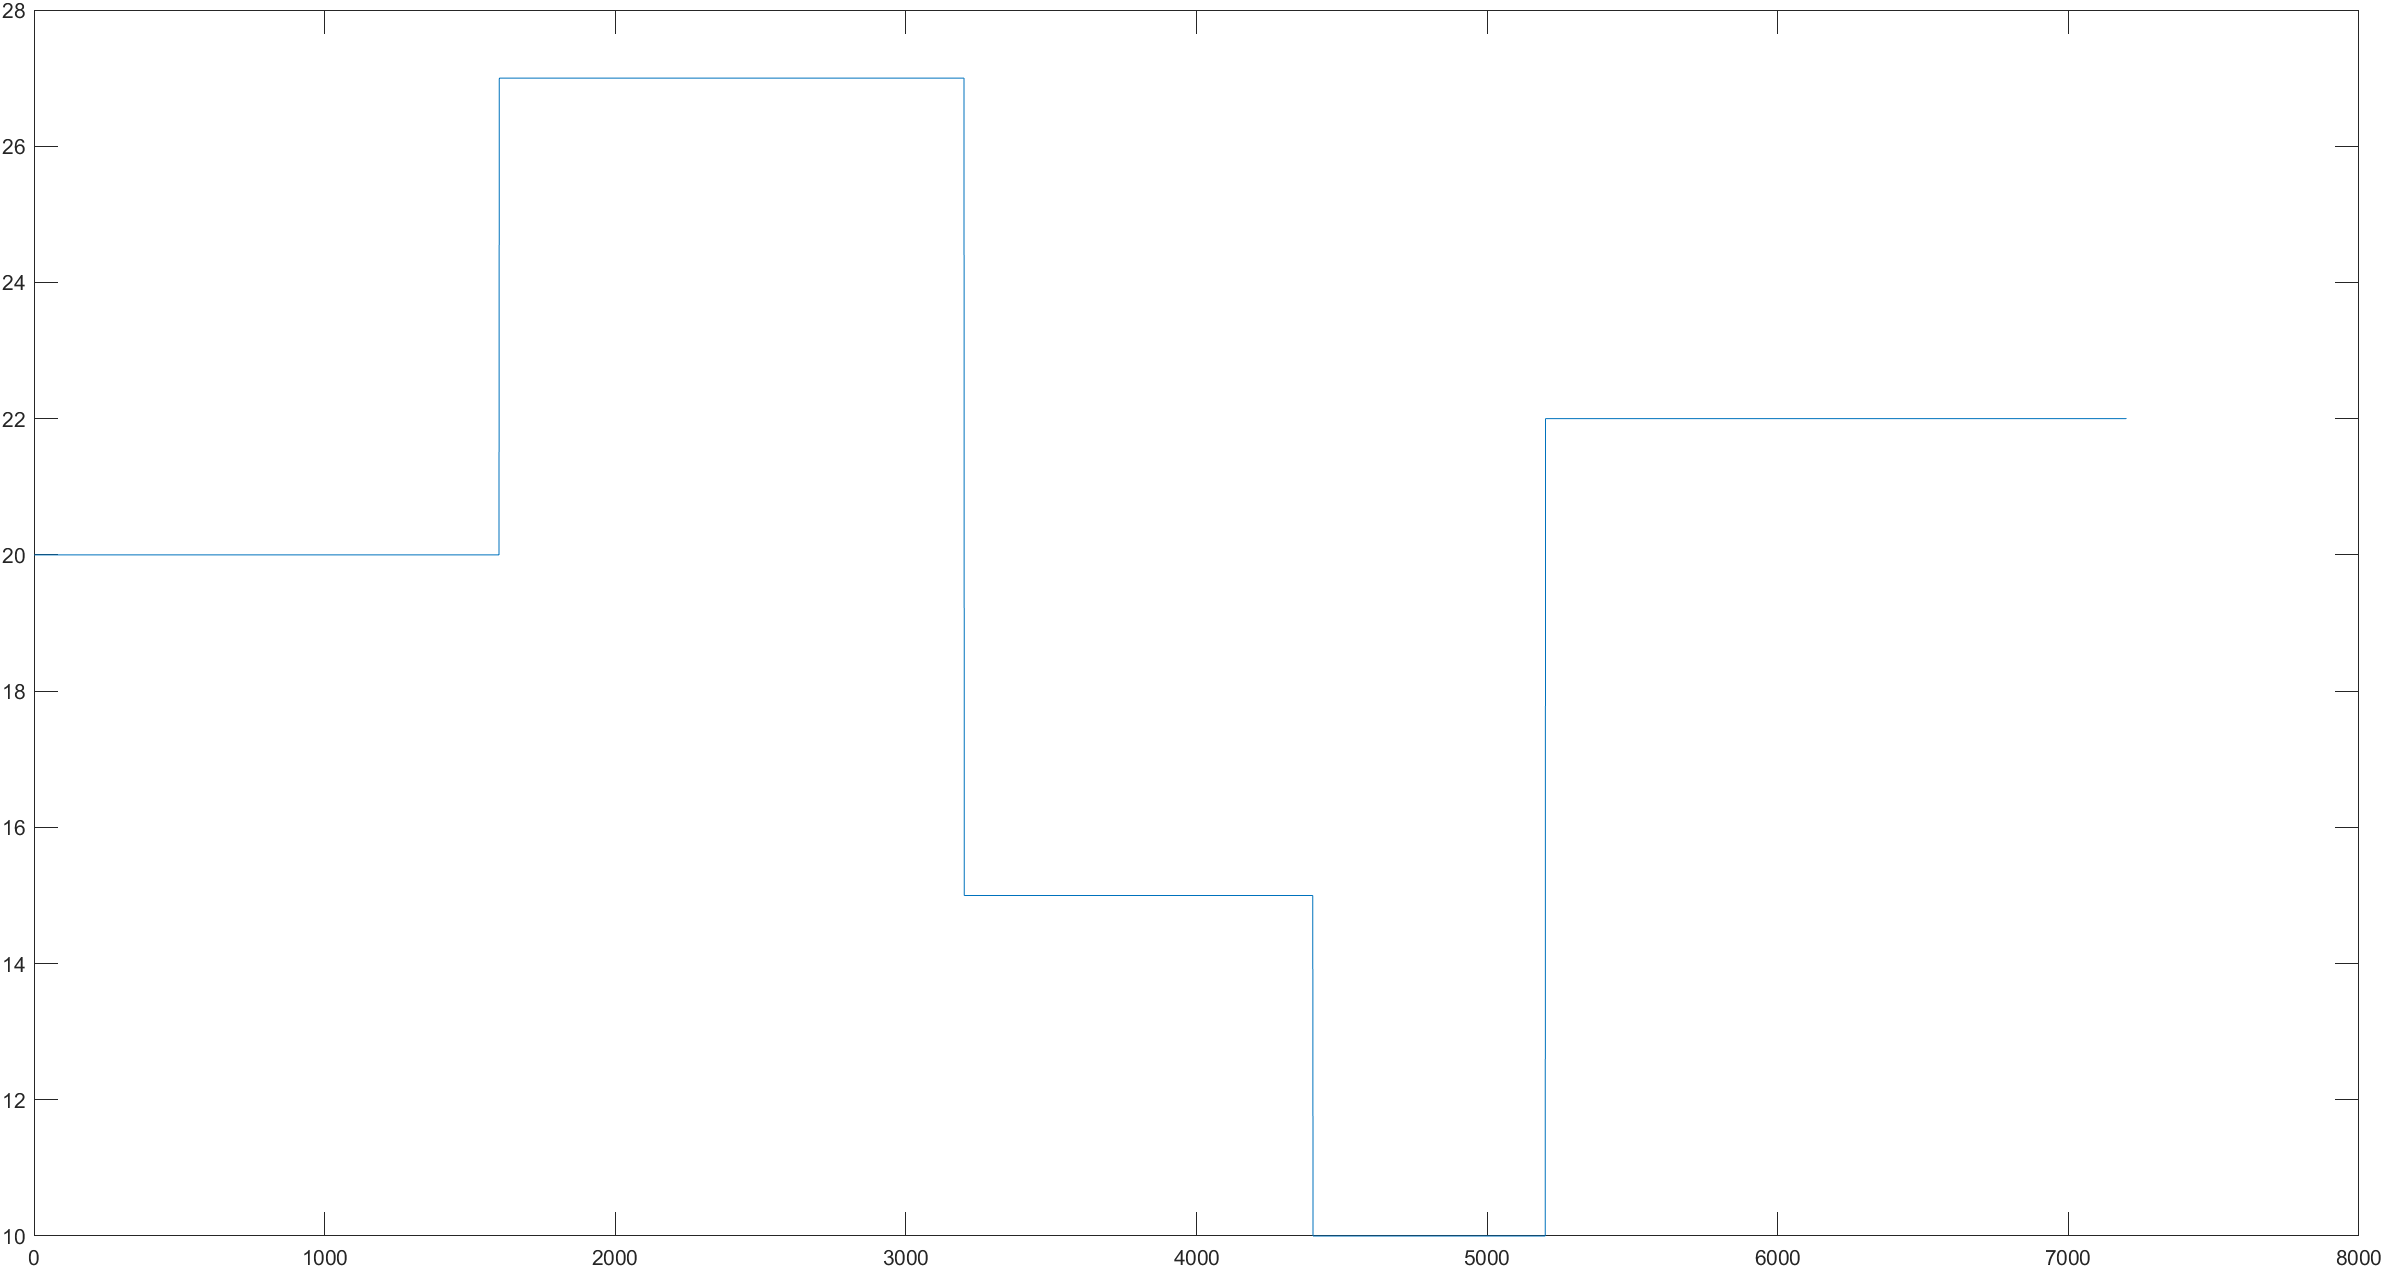
\includegraphics[width=\linewidth]{./pic/input}
	\caption{Simulation Input}
	\label{fig:siminput}
\end{figure}

\par\noindent
Figure \ref{fig:siminput} visualizes how a track profile might look like. It stipulates the maximum allowed velocity for discrete points in time, as well as the overall duration of the simulation; the train either brakes or accelerates accordingly in order to match the corresponding value. An example: Let the simulation time be 1200 seconds, and $v_{max}(1200)=20 \; \frac{m}{s}$. Let the train's velocity $v$ be $25 \; \frac{m}{s}$. The train will engage its brakes (or continue braking, if they have already been engaged) in order to bring $v$ down to $20 \; \frac{m}{s}$. If $v$ were $15 \; \frac{m}{s}$, the train would accelerate instead. The track profile is one of many input parameters, all of which determine the course of the simulation. 

\section{Matlab Code}
\label{sec:MatlabCode}
\par\noindent
A matlab script is used to configure the simulation input, execute the simulation, and write the simulation output into a tabulator-separated file. At the start of execution, the workspace (where variables are stored) should be cleared. Also, the number of cores to use for parallel processing must be set (more on this later):

\bigskip
\begin{python}
clear all
clc
warning ('off','all');
numcores = 10;
\end{python}
\bigskip

\noindent
Generally speaking, simulation input can be divided into two categories: static and dynamic parameters. They, for the most part, correspond to the constants and variables defined in chapter \ref{chap:FundamentalsOfRailwayVehicleEngineering}. The static parameters, i.e. constants, remain the same for every single simulation run, while the dynamic parameters, i.e. variables, may be different for any two simulation runs.

\bigskip
\begin{python}
RBD = 5; 
VBD = 3.5; 
l = 18; 
c = 250; 
\end{python}
\bigskip

\noindent
These constants all correspond to the brake pipe ${\mathcal{M}}_{bp}$, where $RBD$ is the regular operations pressure (i.e. the pressure on the brake pipe when brakes are disengaged), $VBD$ is the full breaking pressure (i.e. the pressure on the brake pipe when brakes are fully engaged), $l$ is the physical length of the brake pipe $l_{bp}$ (although $l_{bp}$ is defined as a variable in ${\mathcal{M}}_{bp}$, it is assumed all wagons have the same physical length for the sake of simplicity), and $c$ is the propagation velocity of the pipe's medium $v_{bp}$.

\bigskip
\begin{python}
tf = 4;
tl = .1;
\end{python}
\bigskip

\noindent
\TODO{}

\bigskip
\begin{python}
p0 = 0;
Pres = 0/1000*[5.7/771 0 1.6];
alpha = 0.9;
BPnum = [0.3 alpha];
BPden = [1 alpha];
\end{python}
\bigskip

\noindent
\TODO{}
\par\noindent
All static parameters have now been initialized. They, along with the track profile, will remain unchanged for all simulations; what sets any two simulations apart is their variable input parameters.

\bigskip
\begin{python}
tmax = 3600;
nmax = tmax * 2;
t = linspace(0, tmax, nmax);
u = [10*ones(1000*2,1); 15*ones(500*2,1); 25*ones(1200*2,1); 12*ones(600*2,1); 0*ones(300*2,1)];
simin.time = t;
simin.signals.values = u;

trackgradient = 0;
\end{python}
\bigskip

\noindent
The code above shows the definition of the track profile. \pyth{tmax} specifies the duration of the simulation in seconds, so in this case one hour. \pyth{nmax} is number of discrete data points; with \pyth{nmax = tmax * 2}, there are on average two data points for every one second of simulation time. \pyth{t} is a linearly spaced vector, i.e. a vector of \pyth{nmax} evenly spaced points between 0 and \pyth{tmax}, which is then set as time input using \pyth{simin.time = t;}. \pyth{u} is the vector which holds the data points, with the number of data points being equal to the value of \pyth{nmax}. The data points stipulate the maximum allowed velocity $v_{max}$ for every discrete point in time. For example, \pyth{10*ones(1000*2,1);} means that for the first 2000 points in time, or for the first 1000 seconds of simulation time, the value of $v_{max}$ is $10 \; \frac{m}{s}$. Continuing with the above example, $v_{max}$ then increases to $15 \; \frac{m}{s}$ for the next 1000 points in time, or the next 500 seconds of simulation time. This vector \pyth{u} is then set as input signal using \pyth{simin.signals.values = u;}. Finally, \pyth{trackgradient = 0;} specifies the average gradient of the track (in this case, the track neither goes uphill, nor downhill).
\par
The goal is to create large quantities of data, i.e. at least hundreds of gigabytes. Since one single simulation run takes, on average, five seconds to complete, and one simulation run produces approximately one megabyte of output data, producing 500 gigabytes worth of data would take 2,500,000 seconds, or almost 29 days. Obviously, this is not acceptable. Fortunately, simulink simulations may be run in parallel, where hardware is the limiting factor rather than time. Albeit, simulations are very expensive, and one will quickly run out of memory if too many simulations are run simultaneously (Using 20 cores, i.e. running 20 simulation in parallel, lead to the server freezing up). Using too many cores also lead to the matlab engine timing out, though whether this was due to memory restrictions or limitations of the engine is unclear. Anyway, using ten CPU cores for parallel processing proved to be stable.

\bigskip
\begin{python}
wagons = 1:1:40;
friction = 0.05:0.01:0.78;
tracforce = 200000:1000:400000;
track = 1;
allruns = 1;
for i = length(tracforce):-1:1
	for j = length(friction):-1:1
		for k = length(wagons):-1:1
			in(track) = Simulink.SimulationInput('Simulation_v2');
			in(track) = in(track).setVariable('num_wagons',wagons(k));
			in(track) = in(track).setVariable('fc',friction(j));
			in(track) = in(track).setVariable('Ft',tracforce(i));
			
			in(track) = in(track).setVariable('alpha',alpha);
			in(track) = in(track).setVariable('BPden',BPden);
			in(track) = in(track).setVariable('BPnum',BPnum);
			in(track) = in(track).setVariable('c',c);
			in(track) = in(track).setVariable('l',l);
			in(track) = in(track).setVariable('nmax',nmax);
			in(track) = in(track).setVariable('p0',p0);
			in(track) = in(track).setVariable('pool',pool);
			in(track) = in(track).setVariable('Pres',Pres);
			in(track) = in(track).setVariable('RBD',RBD);
			in(track) = in(track).setVariable('simin',simin);
			in(track) = in(track).setVariable('t',t);
			in(track) = in(track).setVariable('tf',tf);
			in(track) = in(track).setVariable('tl',tl);
			in(track) = in(track).setVariable('tmax',tmax);
			in(track) = in(track).setVariable('trackgradient',trackgradient);
			in(track) = in(track).setVariable('u',u);
			in(track) = in(track).setVariable('VBD',VBD);
			
			Ft(track) = tracforce(i);
			fc(track) = friction(j);
	
			track = track + 1;        
		end
	end
\end{python}
\bigskip

\par\noindent
 For this purpose, we need to create an array to hold input for all simulation runs. There are three variables which change for each run, they are traction force of the locomotive, wheel/rail friction coefficient and number of wagons, respectively. A nested loop is used to create all possible combinations of these variables, and each single combination gets stored, as a new entry, in the array which holds all input.
\par
Variable ranges are from one to 40 for number of wagons, .05 to .78 for friction coefficient and 200000 to 400000 for traction force, with step sizes one, .01 and 1000 respectively. We therefore have a total number of $40*74*200 =  592000$ combinations. The obvious approach here would be to generate the full batch of 592000 input configurations, but performance and hardware limitations proved this to be unfeasible. Instead, we use rather small batche sizes of 2960 for parallel simulation.
\par
Writing of the output is also done in smaller batches. The best approach to minimize the number of file accessions is of course writing everything into one big matrix, thus storing in RAM, and then writing the matrix in one go. Unfortunately, growing an array by assignment or concatenation can be expensive. For large arrays, MATLAB must allocate a new block of memory and copy the older array contents to the new array as it makes each assignment. The other extreme would of course be to write every single output line directly, but the large number of file accessions required makes this even more unfeasible, so a middle ground is needed, and a batch size of ~3000 works relatively well, although this could surely be optimized with a bit of runtime analysis.
\par
The function below compresses all output of one single simulation into one matrix. Raw simulation output consists of a few time-series objects, like braking force and braking pressure, as well as some metadata. These objects are fed into the write function, which does as many loops as there are rows in the time-series objects. It then packs all rows from each time-series into one big row, adds the meta-data and appends the large row to the matrix, which gets returned at the end. Refer to section \ref{sec:DataStructure} for a more detailed look at the structure of the output matrix.

\begin{matlab}
function ret = Write(id,velocity,force,pressure,distance,acceleration,wagon_ids,t,u,grad,ft,fc)
	numrows = get(force,'Length');
	wagon_ids = double(wagon_ids);
	time = force.Time;
	matrix = [];
	
	for i = 1:1:numrows
		f = getdatasamples(force,i);
		p = getdatasamples(pressure,i);
		v = getdatasamples(velocity,i);
		a = getdatasamples(acceleration,i);
		d = getdatasamples(distance,i);
		
		row = [id,time(i),f,p,v,a,d,wagon_ids,grad,ft,fc]; 	% TODO: add simulation input aka track profile to matrix
		%		print wagon ids as list delimited by colon (,)
		%		performance?
		matrix = [matrix;row];
	end
	fprintf('Created output matrix for simid %d\n',id);
	% writematrix(matrix,'output/output.tsv','FileType','text','WriteMode','append','Delimiter','tab');
	% ret = 1;
	% fprintf('Create output matrix for Simulation ID %d\n', id);
	ret = matrix;
end
\end{matlab}

\begin{python}
import csv
import random

with open('pool.csv', 'w', newline='') as pool:
	fieldnames = ['Wagon_ID', 'Mass', 'Braking_eff']
	writer = csv.DictWriter(pool, fieldnames=fieldnames)
	
	writer.writeheader()
	for i in range(0,500): # create 500 randomized wagons
		mass = random.randrange(12000, 90000, 100) # create random wagon mass between 12 t and 90 t with step size 100
		braking_eff = round(random.uniform(0.75, 0.95),2) # create random braking efficiency as uniform distribution between 75 % and 95 %
		writer.writerow({'Wagon_ID': i, 'Mass': mass, 'Braking_eff': braking_eff})
\end{python}

\par\noindent
The above python script is used to create a randomized pool of 500 wagons to be used in simulation. Each wagon has a unique id, a randomized mass, ranging between 12000 and 90000 kilograms, and a braking efficiency, which is a uniform distribution between .75 and .95.

\section{Data Structure}
\label{sec:DataStructure}
\par\noindent
As has been denoted previously, generated data should be suitable for big data processing. The first approach was to create a new directory for each iteration, and also save the different parameters to different files. Since this is very inefficient in terms of number of file accessions and therefore negatively impacts performance, as well as being unsuitable for transformations to big data file systems like Apache Hadoop or Apache Hive, it has been proposed to write all output into one single file. Let's take a look at the structure first.

\begin{tabular}{|c|c|c|c|c|c|c|c|c|c|c|c|c|c|c|c|c|}
	\hline
	simID & Timestamp & $F_{wagon0}$ & ... & $P_{wagon0}$ & ... & $v_{wagon0}$ & ... & $a_{wagon0}$ & ... & Distance & Wagons & Track angle (tentative) & $F_{t}$ & fc & Track profile \\
	\hline
	&  &  &  &  &  &  &  &  &  &  &  &  &  &  &  &  \\
	\hline
	&  &  &  &  &  &  &  &  &  &  &  &  &  &  &  &  \\
	\hline
	&  &  &  &  &  &  &  &  &  &  &  &  &  &  &  &  \\
	\hline
	&  &  &  &  &  &  &  &  &  &  &  &  &  &  &  &  \\
	\hline
	&  &  &  &  &  &  &  &  &  &  &  &  &  &  &  &  \\
	\hline
	&  &  &  &  &  &  &  &  &  &  &  &  &  &  &  &  \\
	\hline
\end{tabular}

\par\noindent
Some output objects are time-series, namely braking force, braking pressure, acceleration, distance and velocity. Force, pressure and acceleration, which get measured for every wagon, look like this

\begin{tabular}{|c|c|c|c|c|}
	\hline
	Timestamp & $Wagon_{1}$ & $Wagon_{2}$ & ... & $Wagon_{40}$ \\
	\hline
	0 & 0 & 0 & 0 & 0 \\
	\hline
	10 & $x_{1}$ & $x_{2}$ & ... & $x_{40}$ \\
	\hline
	... & ... & ... & ... & ... \\
	\hline
	3600 & $y_{1}$ & $y_{2}$ & ... & $y_{40}$ \\
	\hline
\end{tabular}

\par\noindent
whereas distance and velocity only have two columns and thus look like this

\begin{tabular}{|c|c|}
	\hline
	Timestamp & Value \\
	\hline
	0 & 0 \\
	\hline
	.. & .. \\
	\hline
	3600 & $x$ \\
	\hline
\end{tabular}

\par\noindent
Since they all posses the same number of lines, which is the number of timestamps at which measurements were taken, all columns from all these objects may be compressed into a single table. All columns containing meta-information, for example simulation id, which theoretically only needs to be printed once, get filled with the same value for all lines, and since the number of wagons may vary from one to 40, all possibly empty columns get filled with zeros, so that we do not get any columns containing no value. 

\section{Analysis of generated Data}
\label{sec:AnalysisOfGeneratedData}